\hypertarget{interfaceInt}{
\section{Int  Interface Reference}
\label{interfaceInt}\index{Int@{Int}}
}
Inheritance diagram for Int:\begin{figure}[H]
\begin{center}
\leavevmode
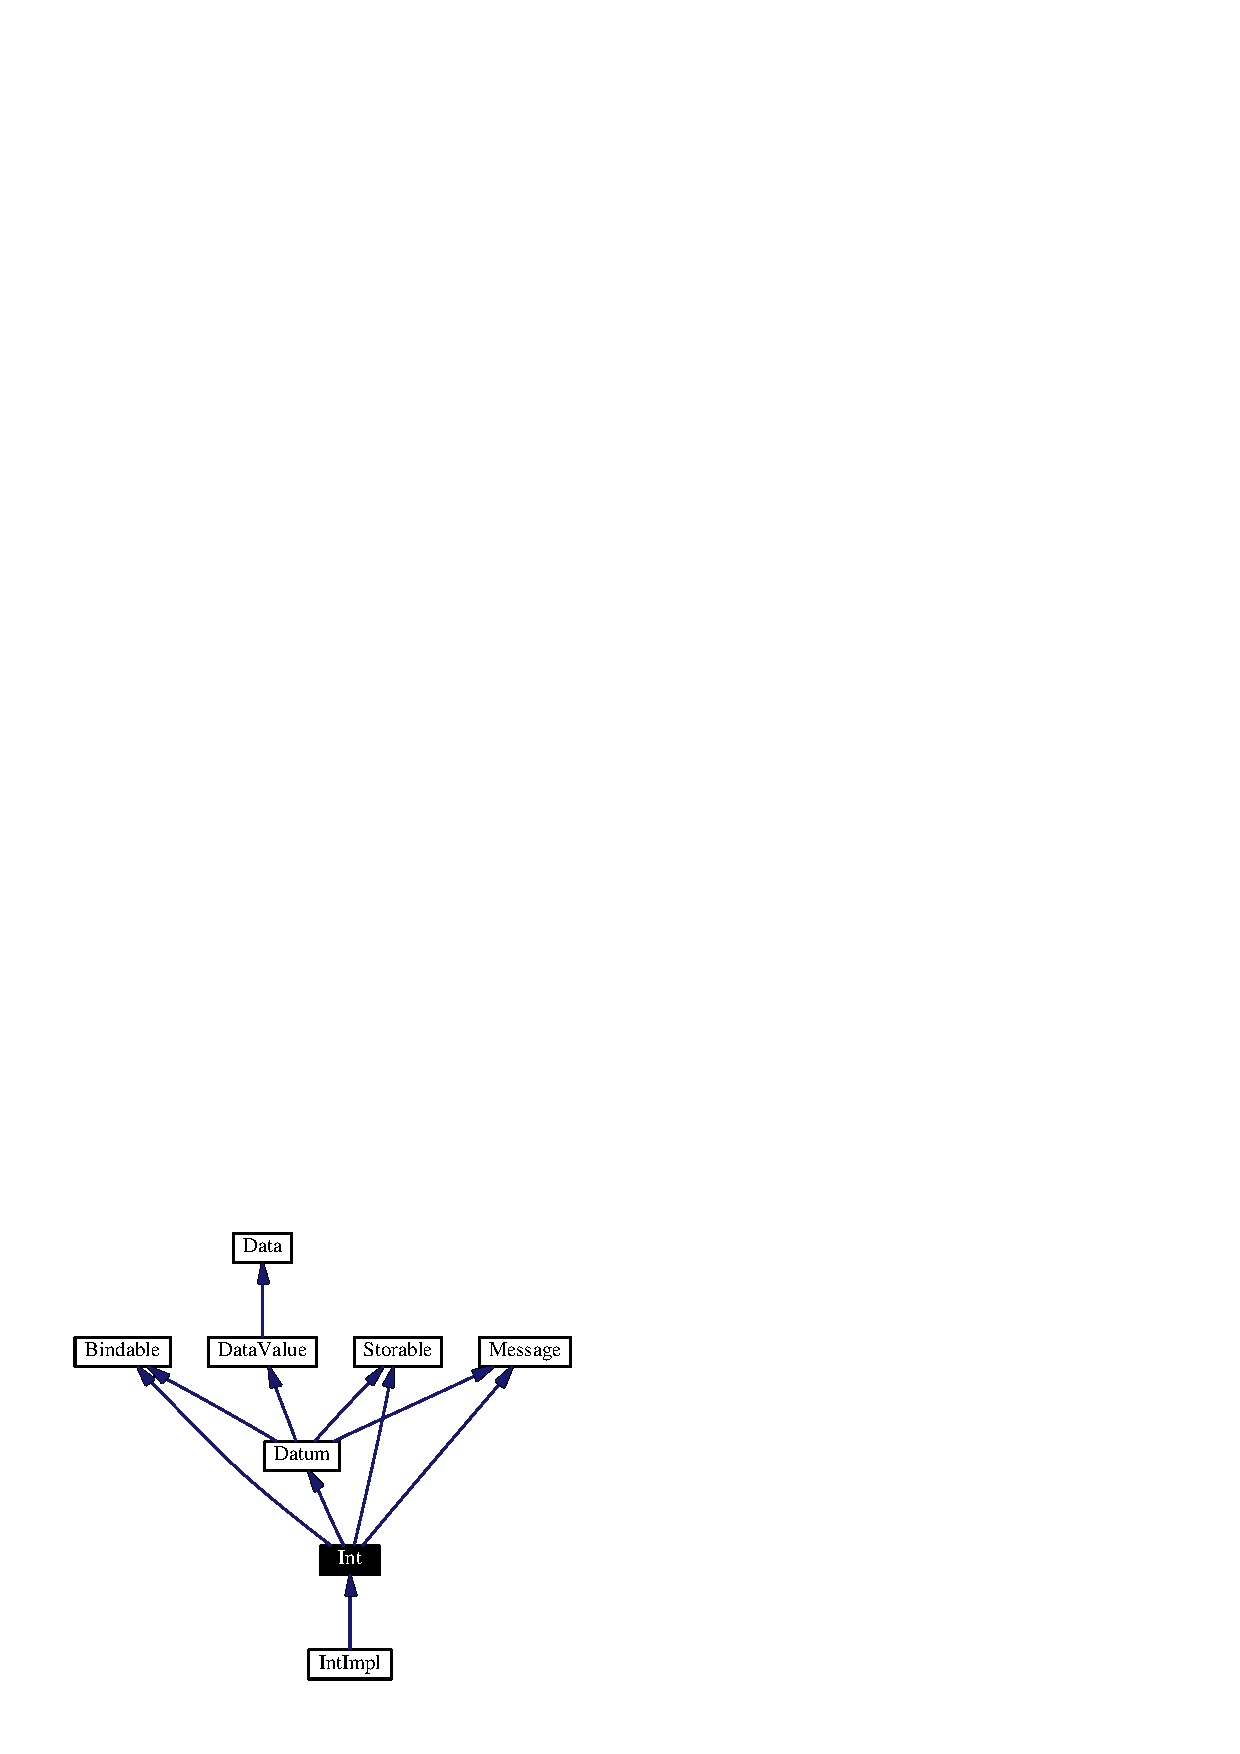
\includegraphics[width=137pt]{interfaceInt__inherit__graph}
\end{center}
\end{figure}
Collaboration diagram for Int:\begin{figure}[H]
\begin{center}
\leavevmode
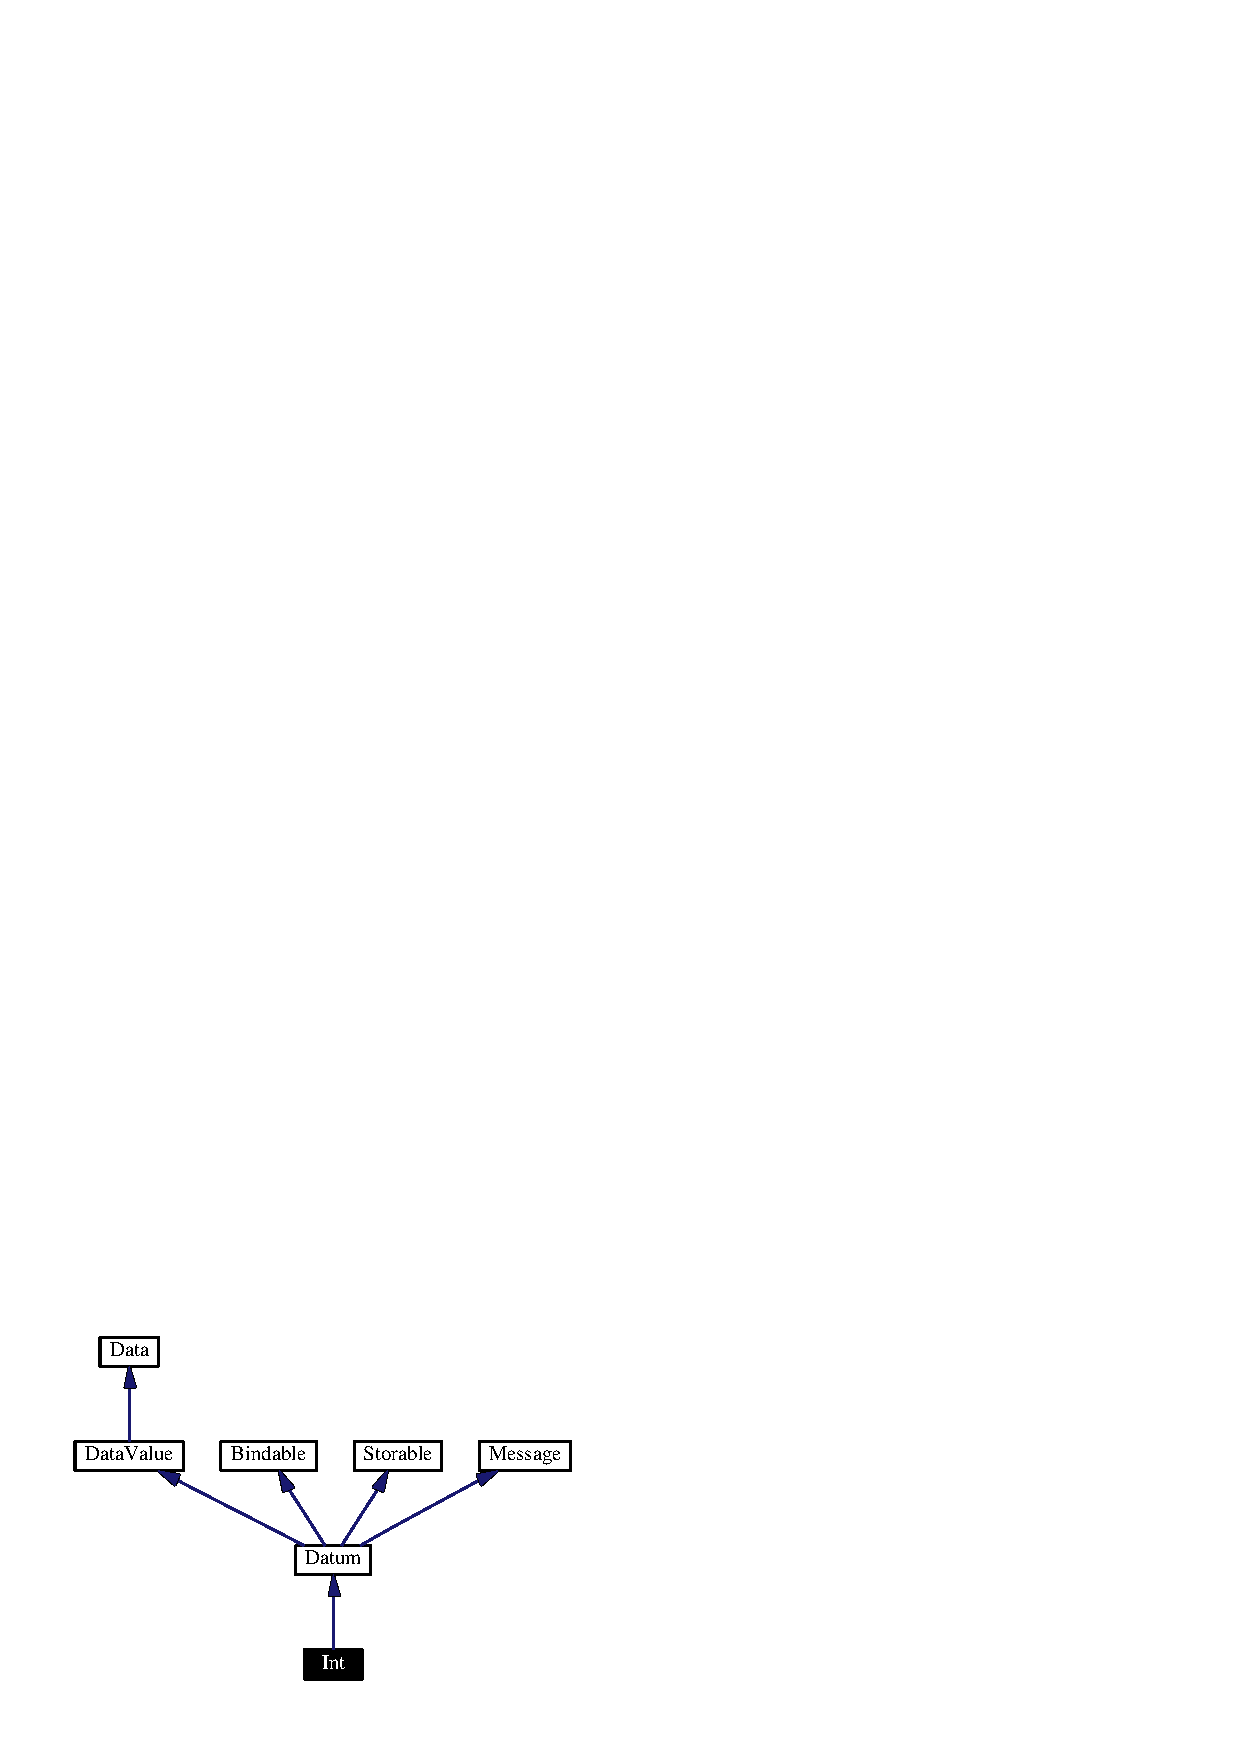
\includegraphics[width=137pt]{interfaceInt__coll__graph}
\end{center}
\end{figure}
\subsection*{Public Methods}
\begin{CompactItemize}
\item 
long \hyperlink{interfaceInt_a0}{int\-Value} ()
\item 
Int \hyperlink{interfaceInt_a1}{plus} (Int n)
\item 
Int \hyperlink{interfaceInt_a2}{minus} (Int n)
\item 
Int \hyperlink{interfaceInt_a3}{monus} (Int n)
\item 
Int \hyperlink{interfaceInt_a4}{times} (Int n)
\item 
\hyperlink{interfaceEmpty}{Empty} \hyperlink{interfaceInt_a5}{greater} (Int n) throws \hyperlink{classExceptional}{Exceptional}
\item 
\hyperlink{interfaceEmpty}{Empty} \hyperlink{interfaceInt_a6}{greater\-Or\-Eq} (Int n) throws \hyperlink{classExceptional}{Exceptional}
\item 
\hyperlink{interfaceEmpty}{Empty} \hyperlink{interfaceInt_a7}{less} (Int n) throws \hyperlink{classExceptional}{Exceptional}
\item 
\hyperlink{interfaceEmpty}{Empty} \hyperlink{interfaceInt_a8}{less\-Or\-Eq} (Int n) throws \hyperlink{classExceptional}{Exceptional}
\end{CompactItemize}


\subsection{Member Function Documentation}
\hypertarget{interfaceInt_a5}{
\index{Int@{Int}!greater@{greater}}
\index{greater@{greater}!Int@{Int}}
\subsubsection[greater]{\setlength{\rightskip}{0pt plus 5cm}\hyperlink{interfaceEmpty}{Empty} Int::greater (Int {\em n})}}
\label{interfaceInt_a5}




Reimplemented in \hyperlink{classIntImpl_a5}{Int\-Impl}.\hypertarget{interfaceInt_a6}{
\index{Int@{Int}!greaterOrEq@{greaterOrEq}}
\index{greaterOrEq@{greaterOrEq}!Int@{Int}}
\subsubsection[greaterOrEq]{\setlength{\rightskip}{0pt plus 5cm}\hyperlink{interfaceEmpty}{Empty} Int::greater\-Or\-Eq (Int {\em n})}}
\label{interfaceInt_a6}




Reimplemented in \hyperlink{classIntImpl_a6}{Int\-Impl}.\hypertarget{interfaceInt_a0}{
\index{Int@{Int}!intValue@{intValue}}
\index{intValue@{intValue}!Int@{Int}}
\subsubsection[intValue]{\setlength{\rightskip}{0pt plus 5cm}long Int::int\-Value ()}}
\label{interfaceInt_a0}




Reimplemented in \hyperlink{classIntImpl_a0}{Int\-Impl}.

Referenced by Int\-Impl::greater(), Int\-Impl::greater\-Or\-Eq(), Int\-Impl::less(), Int\-Impl::less\-Or\-Eq(), Int\-Impl::minus(), Int\-Impl::monus(), Int\-Impl::plus(), and Int\-Impl::times().

\hypertarget{interfaceInt_a7}{
\index{Int@{Int}!less@{less}}
\index{less@{less}!Int@{Int}}
\subsubsection[less]{\setlength{\rightskip}{0pt plus 5cm}\hyperlink{interfaceEmpty}{Empty} Int::less (Int {\em n})}}
\label{interfaceInt_a7}




Reimplemented in \hyperlink{classIntImpl_a7}{Int\-Impl}.\hypertarget{interfaceInt_a8}{
\index{Int@{Int}!lessOrEq@{lessOrEq}}
\index{lessOrEq@{lessOrEq}!Int@{Int}}
\subsubsection[lessOrEq]{\setlength{\rightskip}{0pt plus 5cm}\hyperlink{interfaceEmpty}{Empty} Int::less\-Or\-Eq (Int {\em n})}}
\label{interfaceInt_a8}




Reimplemented in \hyperlink{classIntImpl_a8}{Int\-Impl}.\hypertarget{interfaceInt_a2}{
\index{Int@{Int}!minus@{minus}}
\index{minus@{minus}!Int@{Int}}
\subsubsection[minus]{\setlength{\rightskip}{0pt plus 5cm}Int Int::minus (Int {\em n})}}
\label{interfaceInt_a2}




Reimplemented in \hyperlink{classIntImpl_a2}{Int\-Impl}.\hypertarget{interfaceInt_a3}{
\index{Int@{Int}!monus@{monus}}
\index{monus@{monus}!Int@{Int}}
\subsubsection[monus]{\setlength{\rightskip}{0pt plus 5cm}Int Int::monus (Int {\em n})}}
\label{interfaceInt_a3}




Reimplemented in \hyperlink{classIntImpl_a3}{Int\-Impl}.\hypertarget{interfaceInt_a1}{
\index{Int@{Int}!plus@{plus}}
\index{plus@{plus}!Int@{Int}}
\subsubsection[plus]{\setlength{\rightskip}{0pt plus 5cm}Int Int::plus (Int {\em n})}}
\label{interfaceInt_a1}




Reimplemented in \hyperlink{classIntImpl_a1}{Int\-Impl}.\hypertarget{interfaceInt_a4}{
\index{Int@{Int}!times@{times}}
\index{times@{times}!Int@{Int}}
\subsubsection[times]{\setlength{\rightskip}{0pt plus 5cm}Int Int::times (Int {\em n})}}
\label{interfaceInt_a4}




Reimplemented in \hyperlink{classIntImpl_a4}{Int\-Impl}.

The documentation for this interface was generated from the following file:\begin{CompactItemize}
\item 
\hyperlink{Int_8java-source}{Int.java}\end{CompactItemize}
